% ------------------------------------------------------------------------------
% Resultados
% ------------------------------------------------------------------------------

\chapter{Resultados}\label{chap:resultados}

	O estudo e avaliação do processo de prestação do serviço nos moldes da Engenharia de Sistemas trouxe a clareza necessária para a proposição de sugestões de modificações no
	processo e a inclusão de ferramentas que auxiliam no gerenciamento dos sistemas desenvolvidos. 
	
	Seguindo os procedimentos para coleta de resultados, e aplicando as modificações no processo, foram gerados dados para avaliar o impacto do trabalho realizado, e comparar com medições
	previamente estabelecidas. 

	\section{Resultados para a criação de novas histórias de usuário}

	Ao serem confeccionadas as arquiteturas funcional e física para as novas soluções foram obtidos artefatos de grande importância para as
	fases de \textbf{Desenvolvimento Avançado} e \textbf{Projeto de Engenharia}. No caso da arquitetura física, foi de grande valia para a criação das
	histórias de usuário e tarefas a serem executadas. Nas Figuras \ref{fig:metodologia:solucaoXArqFis} e \ref{fig:metodologia:solucaoYArqFis} vemos as arquiteturas físicas para dois sistemas desenvolvidos seguindo
	a nova metodologia, as caixas de e-mail foram censuradas para preservar o sigilo.

	\begin{figure}[!h]
		\centering
		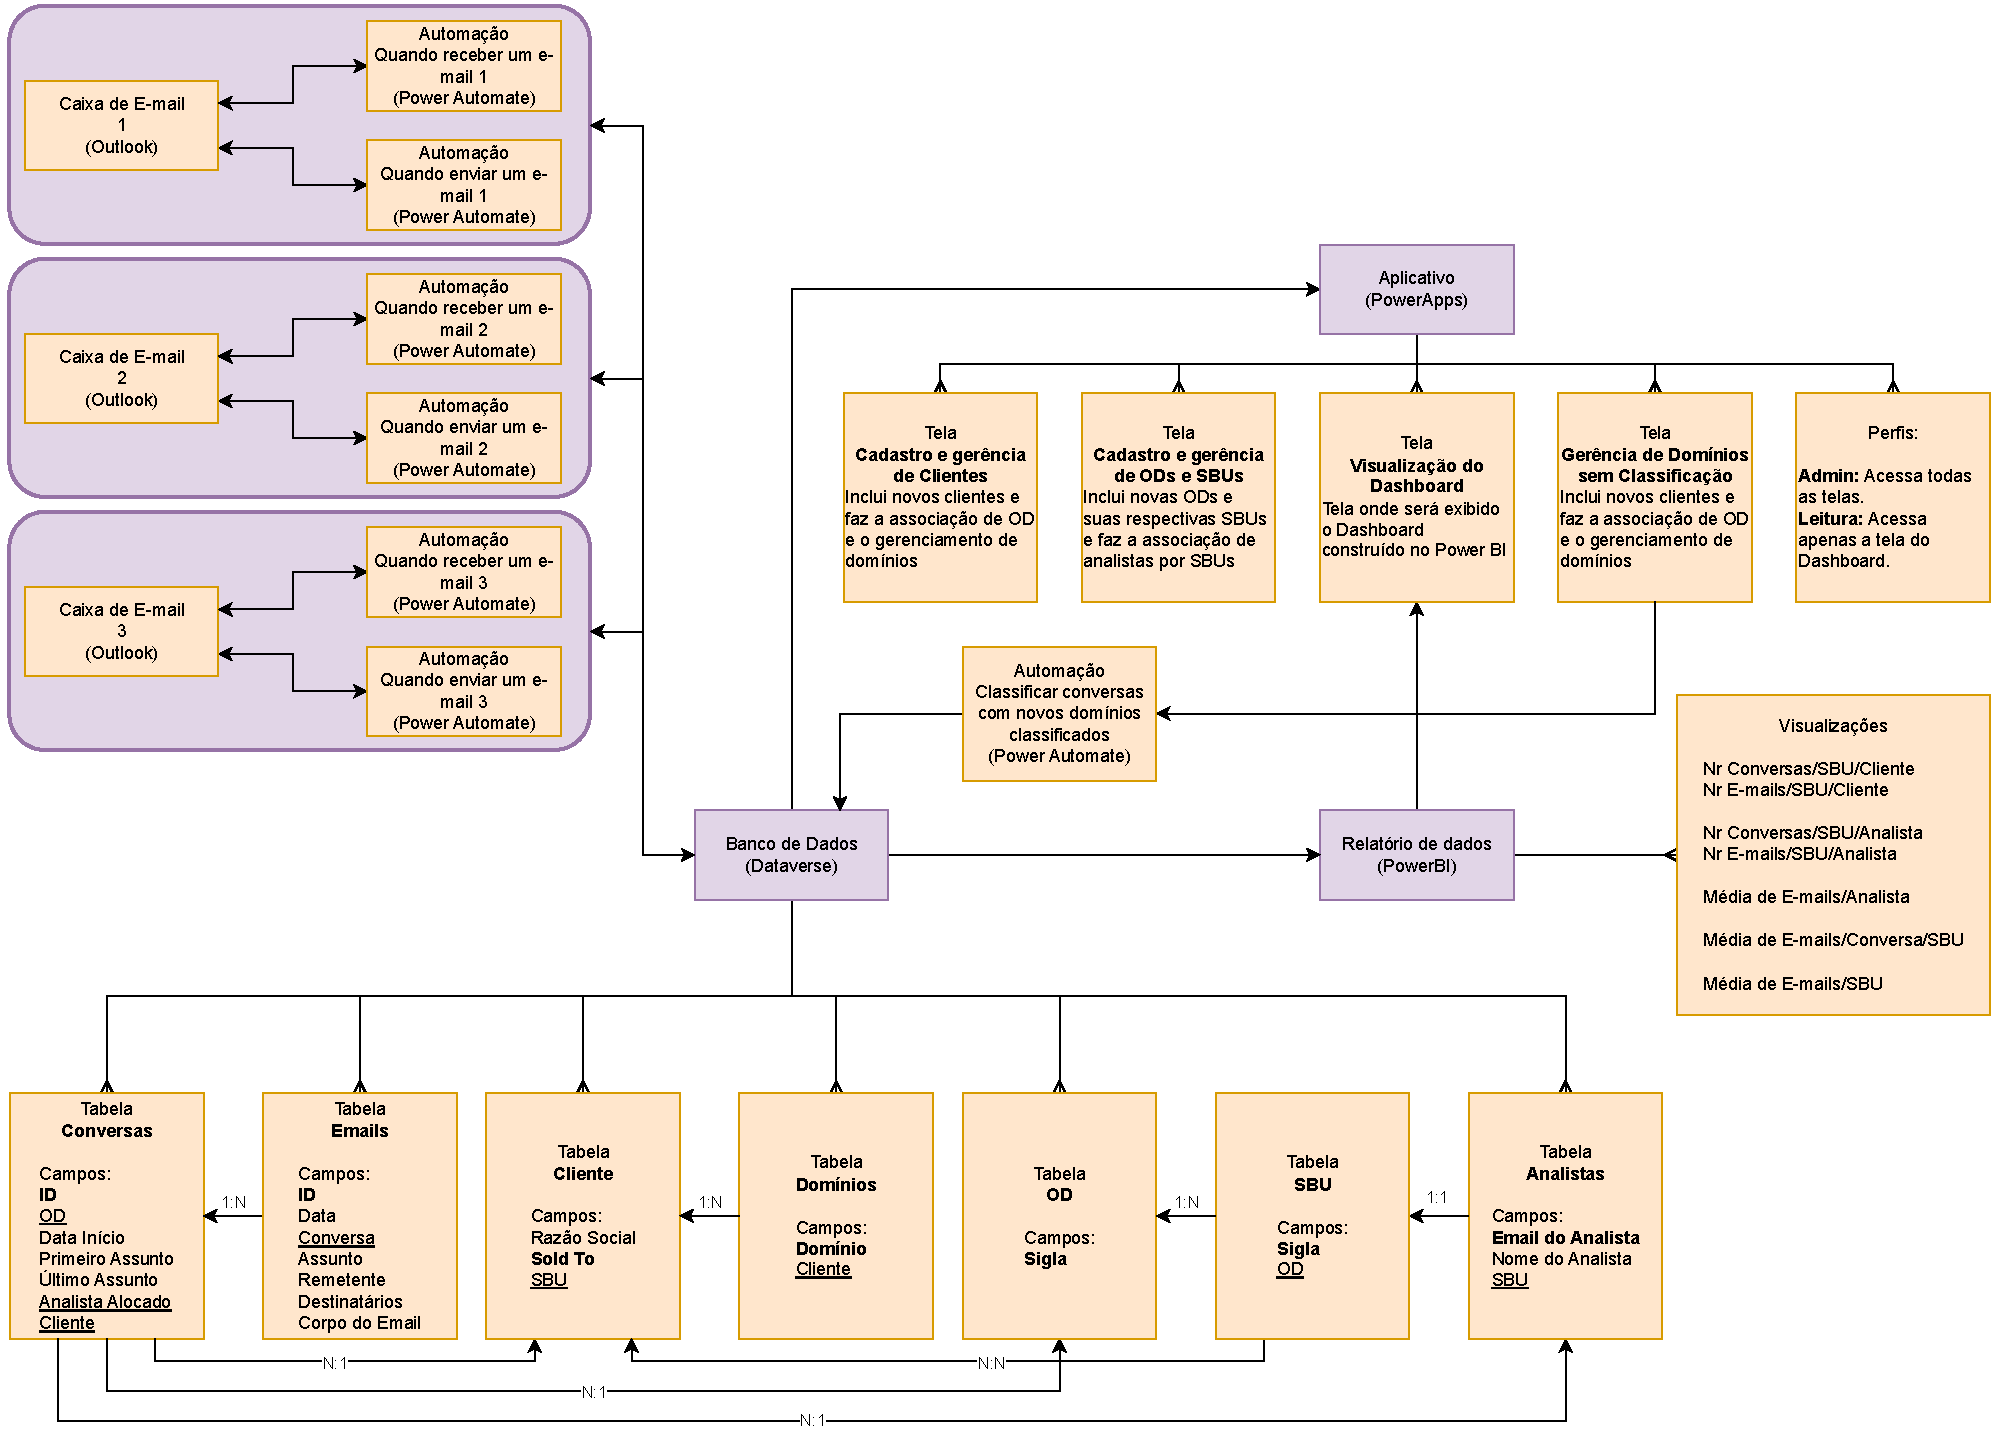
\includegraphics[width=1\textwidth]{./figuras/solucaoXArqFis.pdf}
		\caption{Arquitetura física da Solução X}
		\label{fig:metodologia:solucaoXArqFis}
	\end{figure}
	
	\begin{figure}[!h]
		\centering
		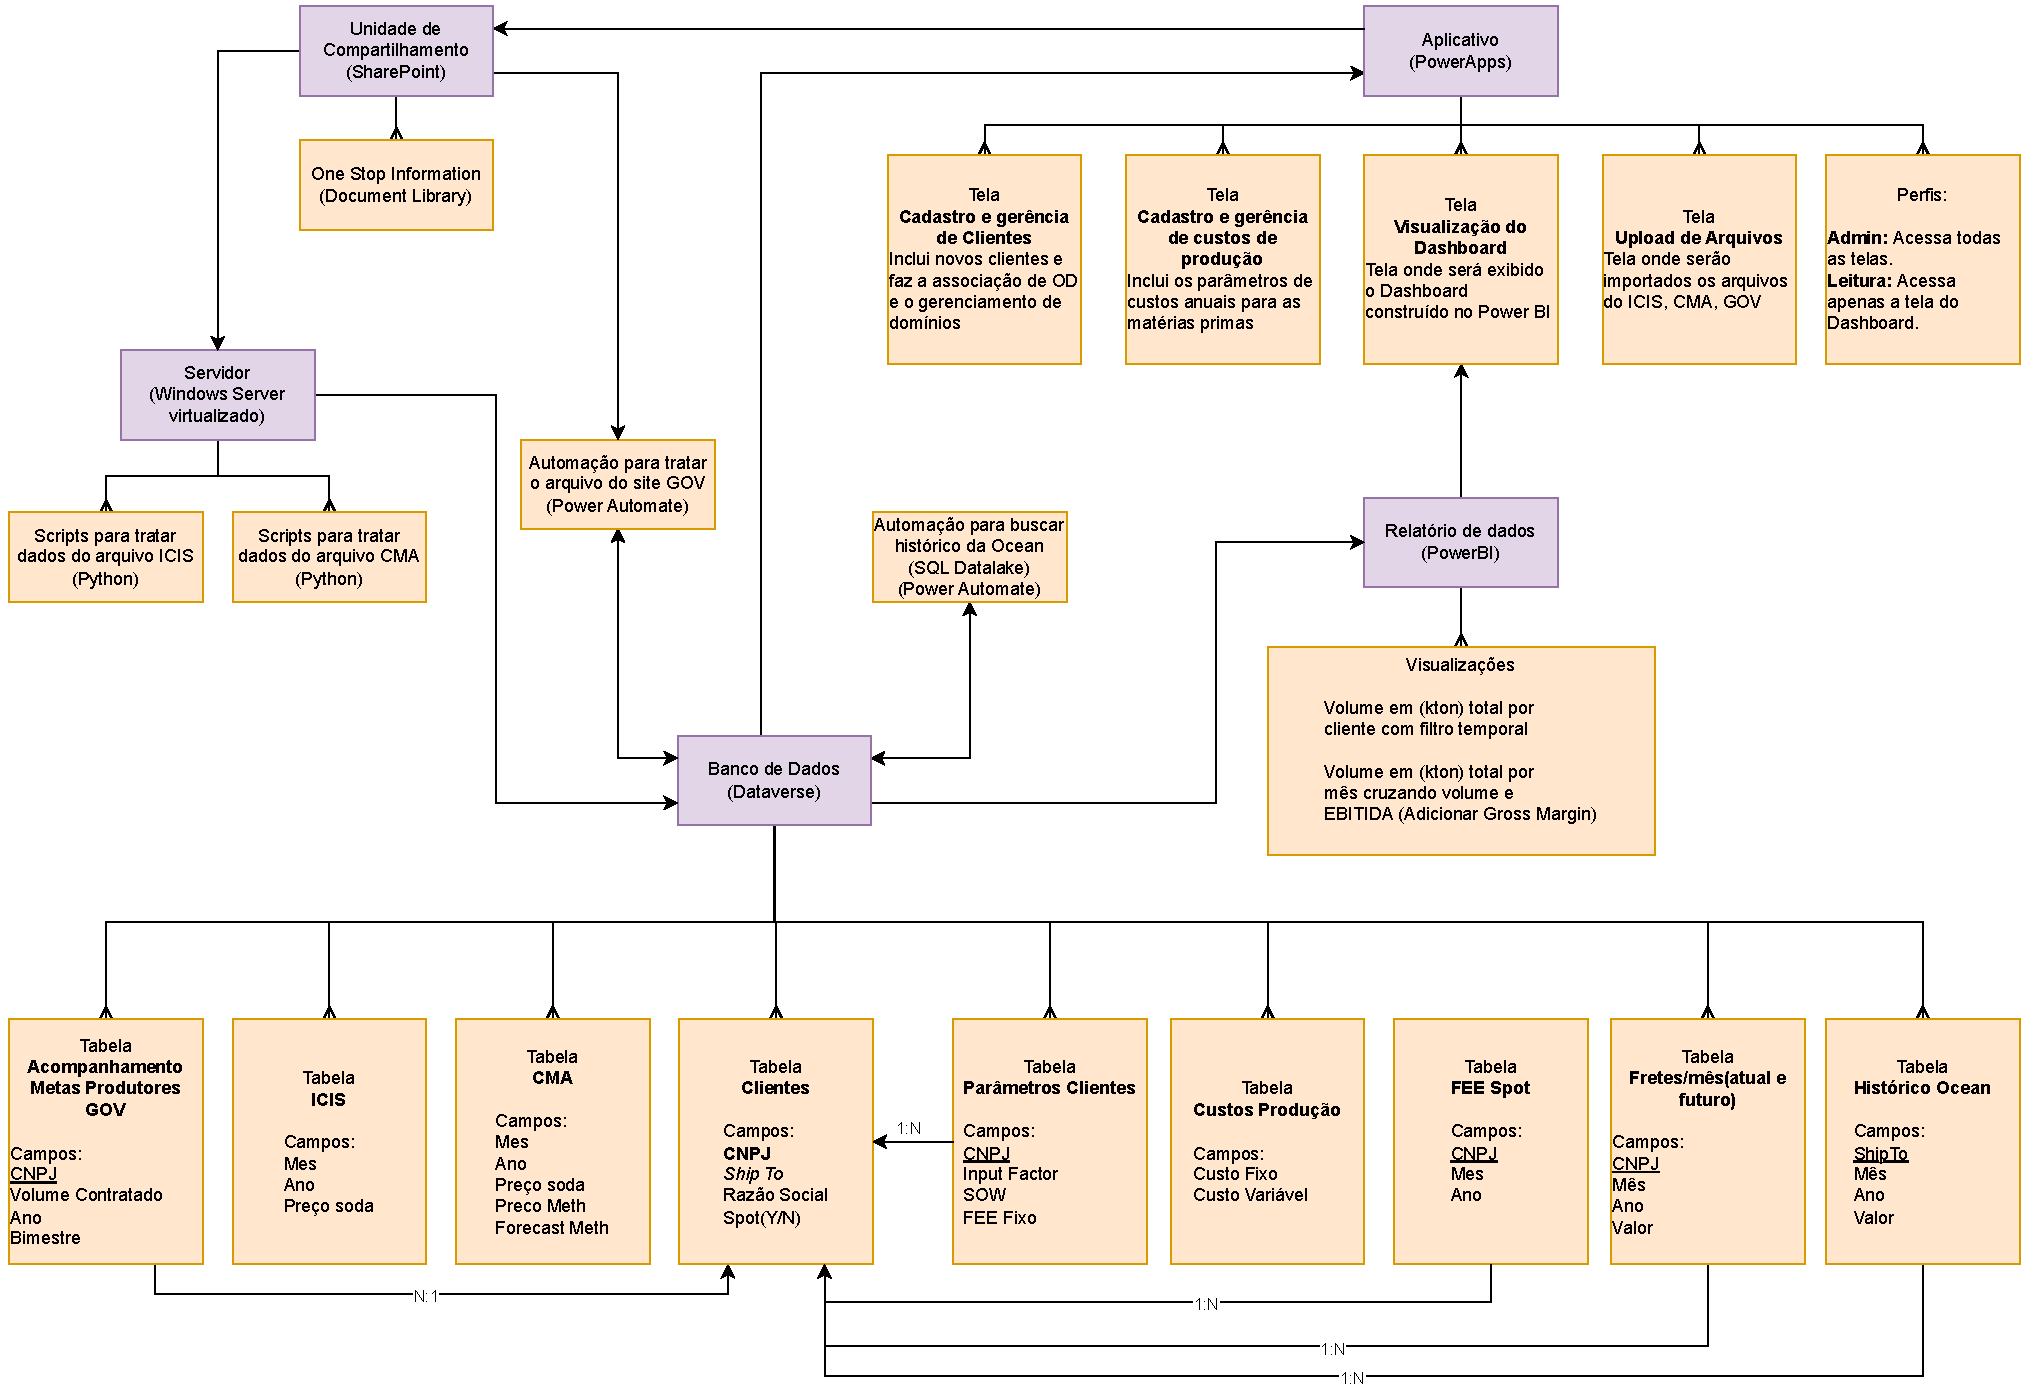
\includegraphics[width=1\textwidth]{./figuras/oneStopArqFis.pdf}
		\caption{Arquitetura física da Solução Y}
		\label{fig:metodologia:solucaoYArqFis}
	\end{figure}

	Baseado nessas arquiteturas, foram criadas as tarefas de cada história de usuário e definido os pontos de esforço. Na Tabela \ref{tab:esforco_solucoes_resultado} foi incluído
	também o aplicativo construído para a rastreabilidade como a Solução Z.

	\begin{longtable}{cccccc}
		\label{tab:esforco_solucoes_resultado} \\
		\toprule
		\textbf{ID} & \textbf{Solução} & \textbf{Categoria} & \textbf{Tarefas} & \textbf{Pontos} & \textbf{Pontos por Tarefa} \\
		\midrule
		\endfirsthead

		\toprule
		\textbf{ID} & \textbf{Solução} & \textbf{Categoria} & \textbf{Tarefas} & \textbf{Pontos} & \textbf{Pontos por Tarefa} \\
		\midrule
		\endhead

		\midrule
		\multicolumn{6}{r}{\textit{continua na próxima página}} \\
		\midrule
		\endfoot

		\bottomrule
		\caption{Distribuição de esforço por solução e categoria}
		\endlastfoot

		178690 & X & Automação & 10 & 10 & 1.00 \\
		178750 & X & Automação & 10 & 10 & 1.00 \\
		178766 & X & Automação & 10 & 10 & 1.00 \\
		178830 & X & Automação & 3 & 5 & 1.67 \\
		179009 & Y & Automação & 2 & 3 & 1.50 \\
		179010 & Y & Automação & 2 & 5 & 2.50 \\
		179011 & Y & Automação & 2 & 2 & 1.00 \\
		178707 & X & Banco de dados & 7 & 13 & 1.86 \\
		179005 & Y & Banco de dados & 12 & 16 & 1.33 \\
		179020 & Z & Banco de dados & 4 & 6 & 1.50 \\
		178825 & X & Relatório de dados & 5 & 15 & 3.00 \\
		179006 & Y & Relatório de dados & 8 & 18 & 2.25 \\
		179007 & Y & Script & 3 & 8 & 2.67 \\
		179008 & Y & Script & 3 & 8 & 2.67 \\
		178784 & X & Tela & 9 & 16 & 1.78 \\
		178795 & X & Tela & 9 & 19 & 2.11 \\
		178806 & X & Tela & 5 & 7 & 1.40 \\
		178814 & X & Tela & 9 & 17 & 1.89 \\
		179001 & Y & Tela & 4 & 12 & 3.00 \\
		179002 & Y & Tela & 5 & 12 & 2.40 \\
		179003 & Y & Tela & 6 & 13 & 2.17 \\
		179004 & Y & Tela & 4 & 5 & 1.25 \\
		179021 & Z & Tela & 3 & 5 & 1.67 \\
		179022 & Z & Tela & 2 & 4 & 2.00 \\
		179023 & Z & Tela & 3 & 5 & 1.67 \\
	\end{longtable}


	\begin{table}[!htb]
		\centering
		\begin{tabular}{ccc}
			\toprule
			\textbf{Categoria} & \textbf{Média de Pontos/Tarefas} & \textbf{Desvio Padrão de Pontos/Tarefas} \\
			\midrule
			Automação          & 1.38                             & 0.57                                 \\
			Banco de dados     & 1.56                             & 0.07                                 \\
			Relatório de dados & 2.63                             & 0.28                                 \\
			Script             & 2.67                             & 0.00                                 \\
			Tela               & 2.00                             & 0.51                                 \\
			\bottomrule
		\end{tabular}
		\caption{Média e variância dos pontos de esforço por categoria após aplicação das mudanças sugeridas}
		\label{tab:media_variancia_resultado}
	\end{table}

	É notável que houve uma queda nas médias de pontos por tarefas em todas as categorias de desenvolvimento ao se comparar com as mesmas estatísticas dos dados históricos mostrados na Tabela
	\ref{tab:media_desvio_historico}. Nota-se também uma queda no desvio padrão de cada categoria, no caso da categoria Script, observa-se um valor nulo, pois as duas atividades de desenvolvimento nessa categoria
	possuíam os mesmos números de tarefas e esforço, e como são, ainda por cima, da mesma solução, não trazem consigo uma representatividade suficiente para serem levados em consideração como um ganho.

	Para as outras categorias, no entanto, esses valores representam uma distribuição mais uniforme de esforço por tarefa e um nível de detalhamento maior. Esse resultado anda paralelo a 
	um melhor entendimento do serviço a ser executado.

	Nas reuniões para validação da solução com as áreas clientes, ou simplesmente a validação de conceito, a arquitetura física foi de grande ajuda para o engajamento do pessoal. As partes interessadas
	foram capazes de opinar e sugerir alterações, visto que o nível de detalhamento apresentado não chegou a um nível inascessível. Além disso, ela funciona como um documento comprobatório do escopo do projeto, evitando  de forma {\color{red} ???}, a
	inclusão de novas fucionalidades fora do escopo, que não estão acomodades no sistema projetado e definido.


	Além dos dados numéricos apresentados, vale ressaltar que com a documentação das arquiteturas funcionais e físicas, foi viabilizado a utilização do auxílio
	do agente de IA autônomo (\textit{Microsoft Copilot}) para a criação das histórias de usuários. Ao serem enviados os documentos das arquiteturas com um \text{prompt} contextualizando sobre a solução e
	a estrutura e ferramentas de trabalho da equipe, o agente foi capaz de gerar as histórias de usuário e suas tarefas com bastante exatidão, e poucas alterações durante a
	revisão das mesmas, basicamente sendo necessária apenas a exclusão de tarefas desnecessárias, a unificação de tarefas pequenas e muito relacionadas, ou a inclusão de poucas tarefas não consideradas.

	\begin{table}[!htb]
		\centering
		\begin{tabular}{cccc}
			\toprule
			\textbf{Solucão} & \textbf{Tarefas Sugeridas} & \textbf{Tarefas Utilizadas} & \textbf{Diferença percentual} \\
			\midrule
			X & 92  & 77 & -16.3\% \\
			Y & 44  & 51 & 13.7\% \\
			Z & 12  & 12 & 0\% \\
			\bottomrule
		\end{tabular}
		\caption{Quantidade de tarefas geradas pelo agente de IA, a quantidade realmente utilizada e a Diferença percentual}
		\label{tab:tarefas_copilot}
	\end{table}
	
	É visto um bom aproveitamento da tarefas sugeridas, e nota-se que para soluções menos complexas o agente autônomo foi mais assertivo nas tarefas a serem executadas. Esse tipo de
	ação e colaboração com IA trás uma economia de tempo e recurso muito significativa, onde antes o desenvolvedor deveria criar toda a estrutura, e agora apenas revisa e faz pequenas alterações,
	sobrando então mais tempo para atividades de desenvolvimento de fato.

	\section{Resultados para Rastreabilidade}

	A proposta de criar uma aplicação para garantir a rastreabilidade do sistema traz valor em fases mais avançadas do ciclo de vida, em especial as fases de utilização e suporte. Caso surja
	alguma melhoria ou manutenção nessas etapas, o custo envolvido nessas mudanças é maior que se fossem feitas durante a fase de produção, no caso o custo é o equivalente ao esforço empenhado nessas
	mudanças. Então, saber exatamente o impacto dessas alterações no sistema se torna crucial para uma ação consciente e responsável.

	O aplicativo construído pode ser observado nas Figuras \ref{fig:resultados:solucoes} a \ref{fig:resultados:dependenciaCruzada}.

	\begin{figure}[!h]
		\centering
		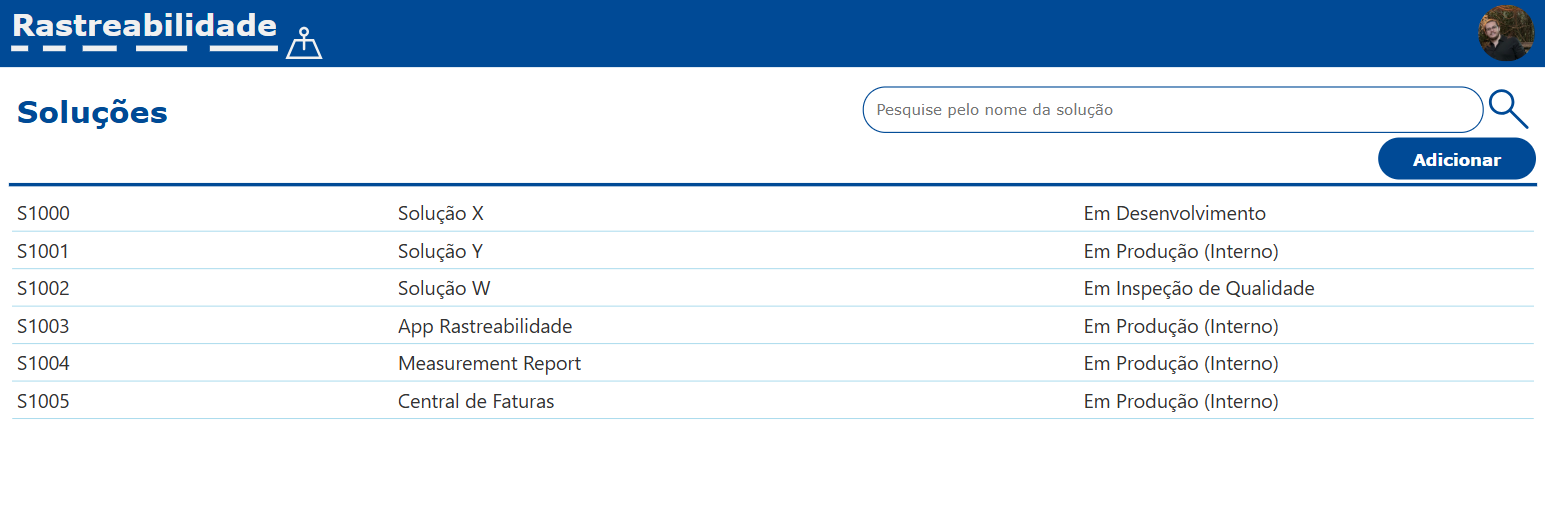
\includegraphics[width=1\textwidth]{./figuras/solucoes.png}
		\caption{Tela de visualização das soluções.}
		\label{fig:resultados:solucoes}
	\end{figure}

	\begin{figure}[!h]
		\centering
		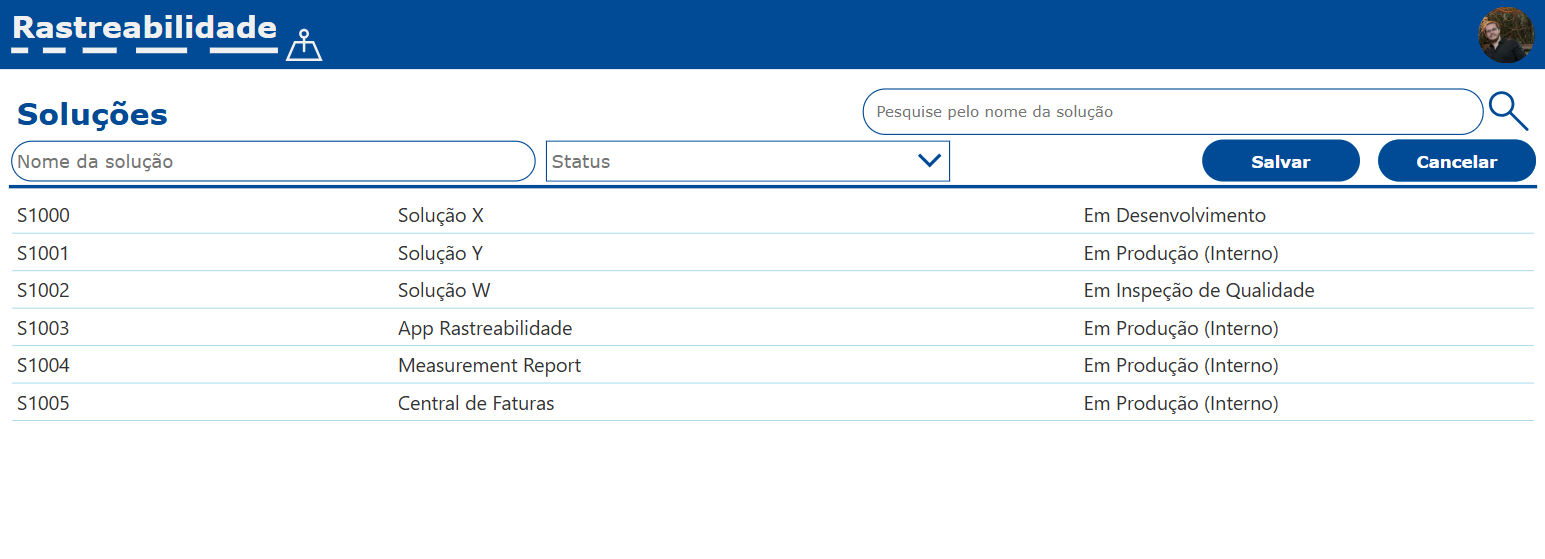
\includegraphics[width=1\textwidth]{./figuras/solucoesAdicionar.png}
		\caption{Tela de visualização das soluções com a expansão dos campos para adicionar nova solução.}
		\label{fig:resultados:solucoesAdicionar}
	\end{figure}

	\begin{figure}[!h]
		\centering
		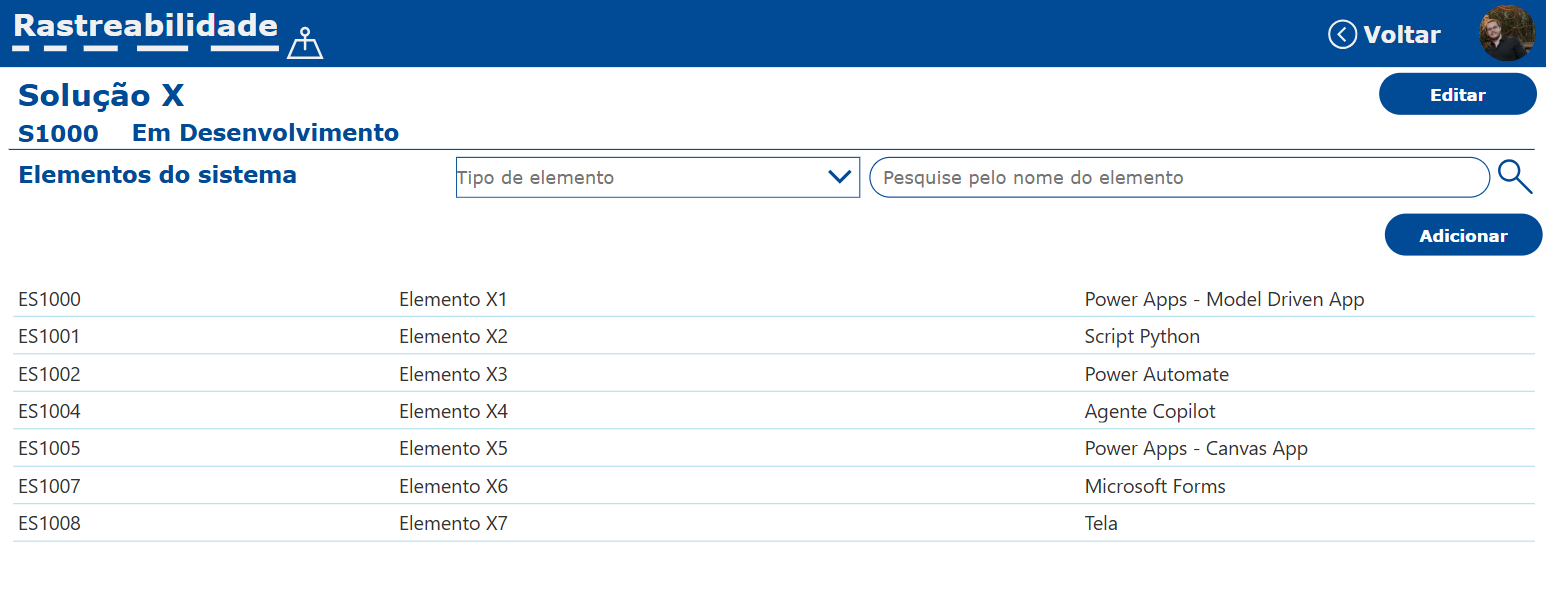
\includegraphics[width=1\textwidth]{./figuras/solucaoElementos.png}
		\caption{Tela de visualização dos elementos.}
		\label{fig:resultados:solucaoElementos}
	\end{figure}

	\begin{figure}[!h]
		\centering
		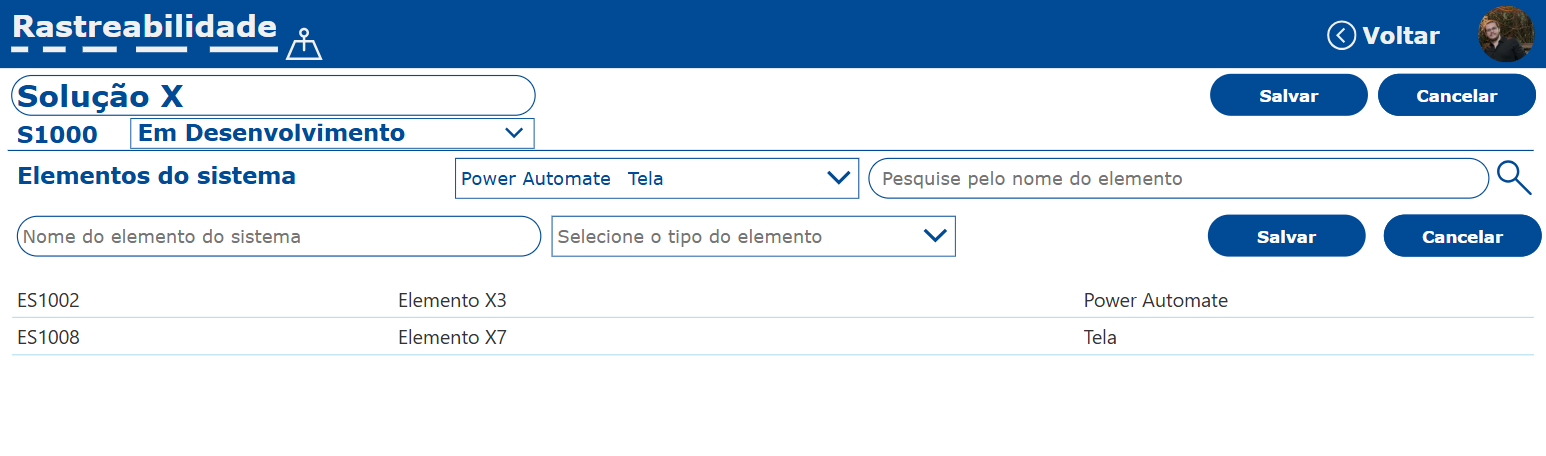
\includegraphics[width=1\textwidth]{./figuras/solucaoElementosAdd.png}
		\caption{Tela de visualização dos elementos com a expansão dos campos para adicionar novo elemento e editar dados da soluçao atual.}
		\label{fig:resultados:solucaoElementosAdd}
	\end{figure}

	\begin{figure}[!h]
		\centering
		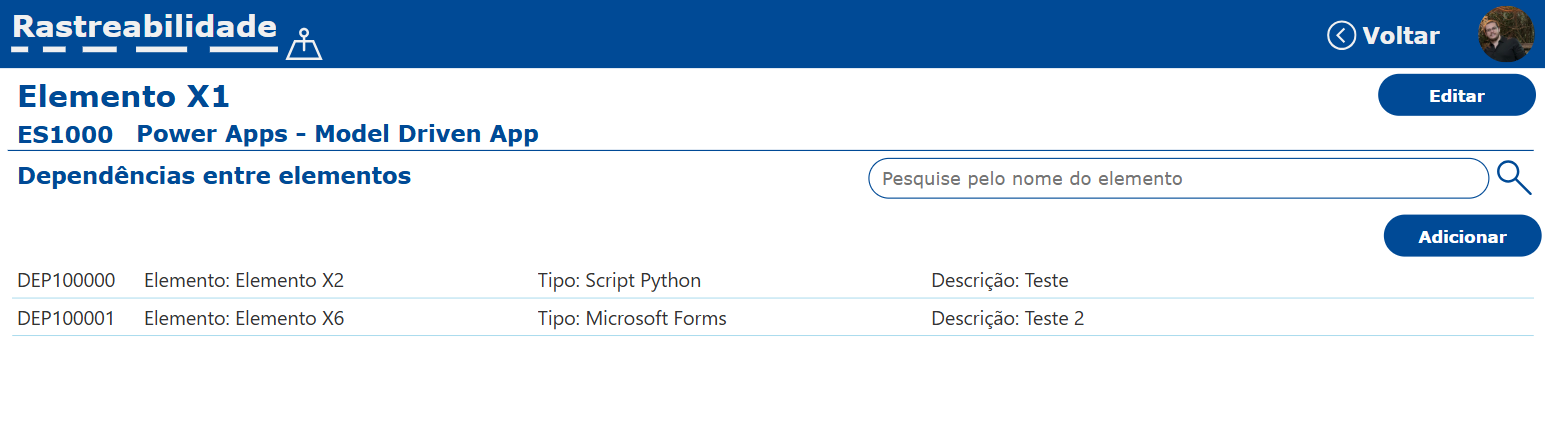
\includegraphics[width=1\textwidth]{./figuras/elementoDependencias.png}
		\caption{Tela de visualização das dependências.}
		\label{fig:resultados:elementoDependencias}
	\end{figure}

	\begin{figure}[!h]
		\centering
		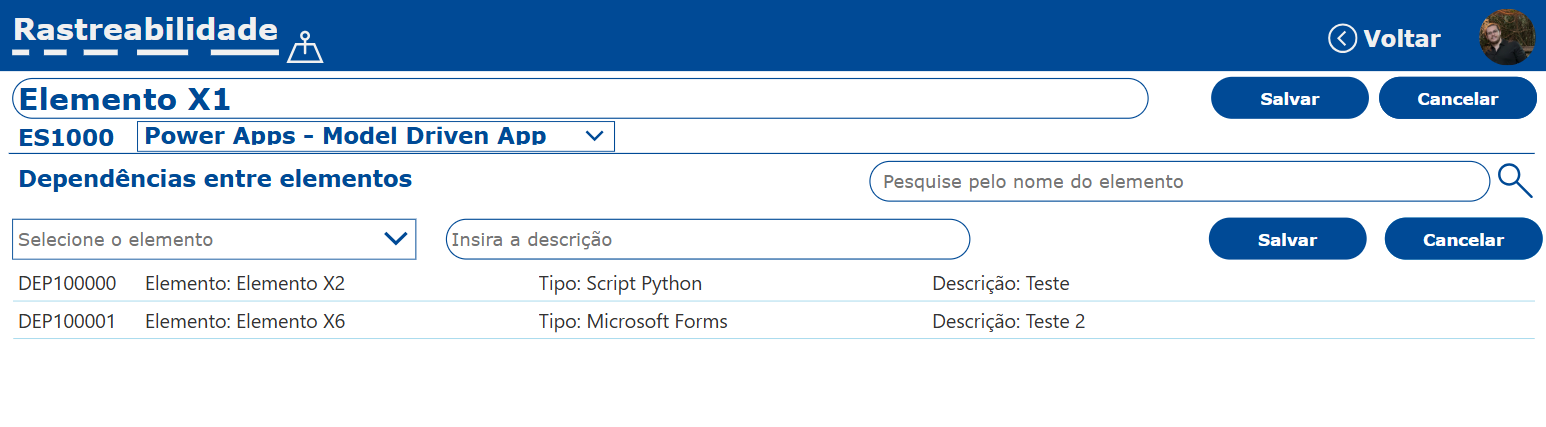
\includegraphics[width=1\textwidth]{./figuras/elementoDependenciasAdd.png}
		\caption{Tela de visualização das dependências com a expansão dos campos para adicionar nova dependência e editar o elemento atual}
		\label{fig:resultados:elementoDependenciasAdd}
	\end{figure}

	\begin{figure}[!h]
		\centering
		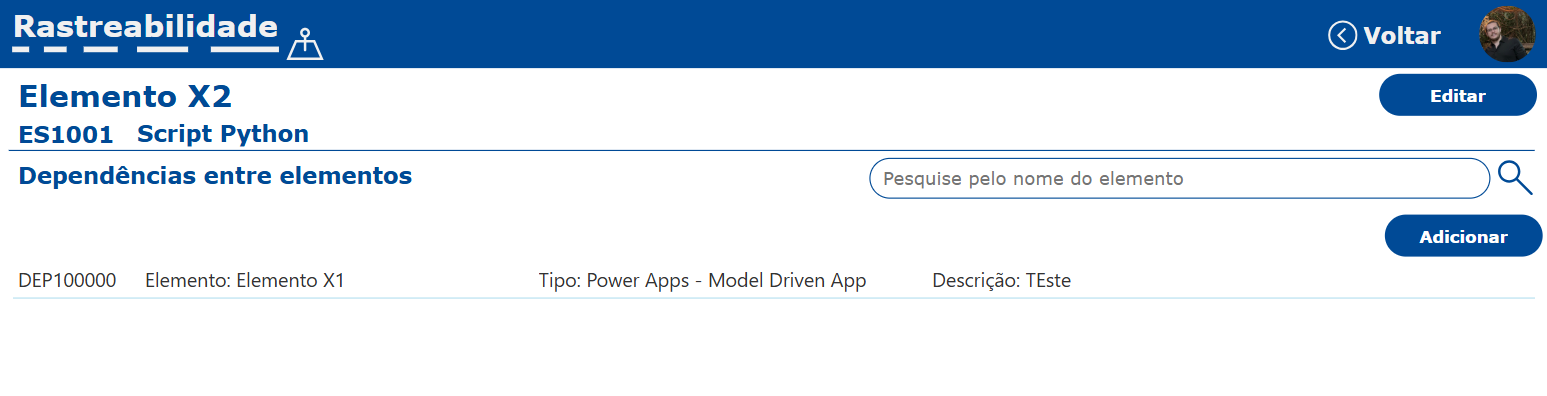
\includegraphics[width=1\textwidth]{./figuras/dependenciaCruzada.png}
		\caption{Tela de visualização evidenciando a dependência cruzada.}
		\label{fig:resultados:dependenciaCruzada}
	\end{figure}

	Como sugerido, foram propostos três cenários para avaliação de esforço de atuação:

	\begin{itemize}
		\item \textbf{Cenário 1:} O fluxo de automação que envia o resultado da análise das notas fiscais para o fornecedor e as notas aprovadas para {\color{red} pamaneto},
		foi deletado por engano e precisa ser feito novamente.
		\item \textbf{Cenário 2:} A caixa compartilhada de e-mail utilizada para as notificações do sistema precisa ser substituída por outra.
		\item \textbf{Cenário 3:} A inclusão de uma coluna com dado importante em uma tabela que deve ser exibida junto com as outras informações provenientes dessa tabela, seja no e-mail ou no próprio aplicativo.
	\end{itemize}

	As imagens \ref{fig:resultados:sendReviewedResponse}, \ref{fig:resultados:caixadeEmail} e \ref{fig:resultados:solicitacoesTabela} mostram as telas do aplicativo
	que foram mostradas para cada cenário antes da reavaliação pelo desenvolvedores.

	\begin{figure}[!h]
		\centering
		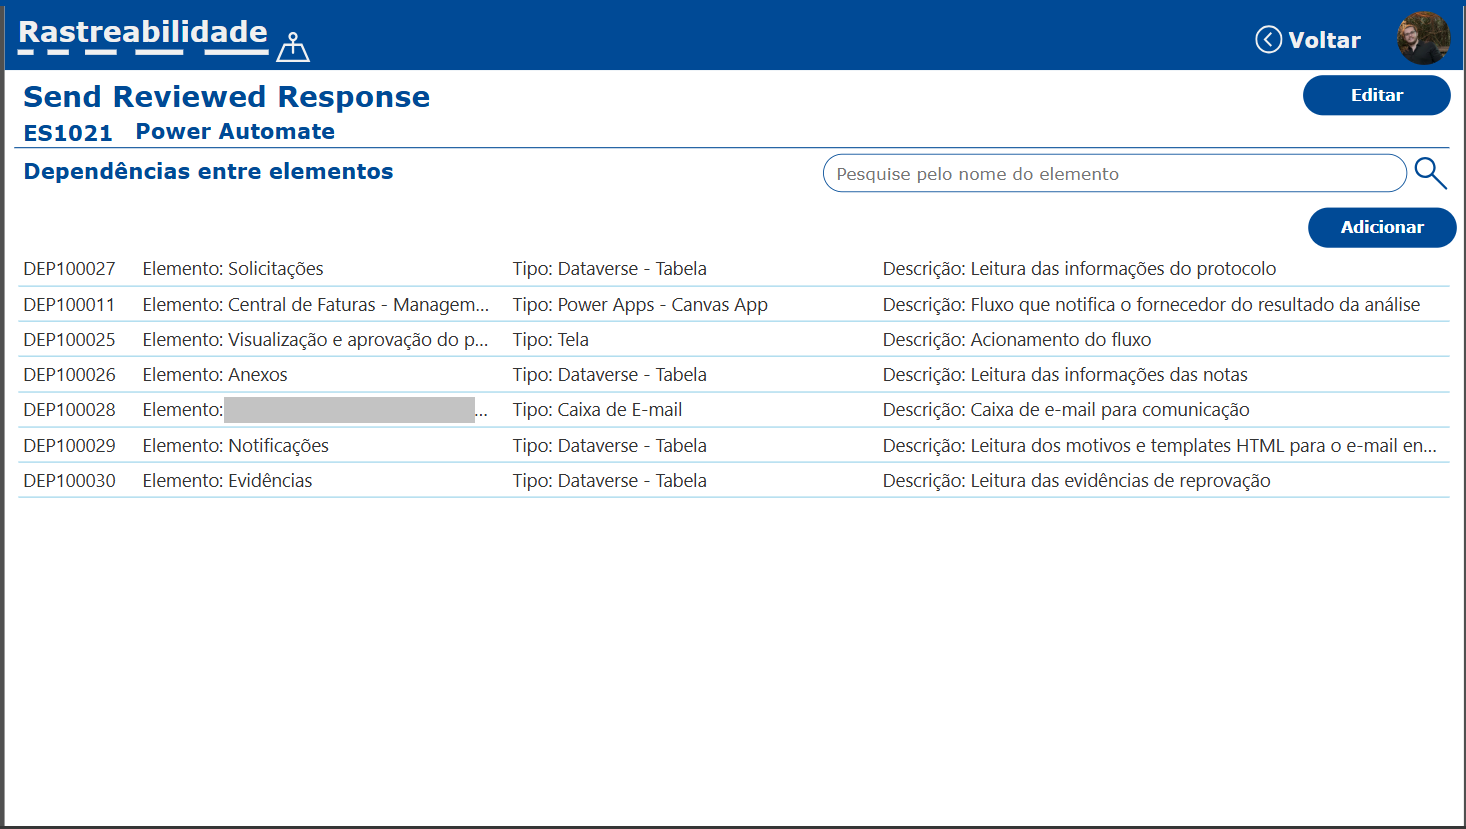
\includegraphics[width=1\textwidth]{./figuras/sendReviewedResponse.png}
		\caption{Dependências relacionadas ao Cenário 1}
		\label{fig:resultados:sendReviewedResponse}
	\end{figure}

	\begin{figure}[!h]
		\centering
		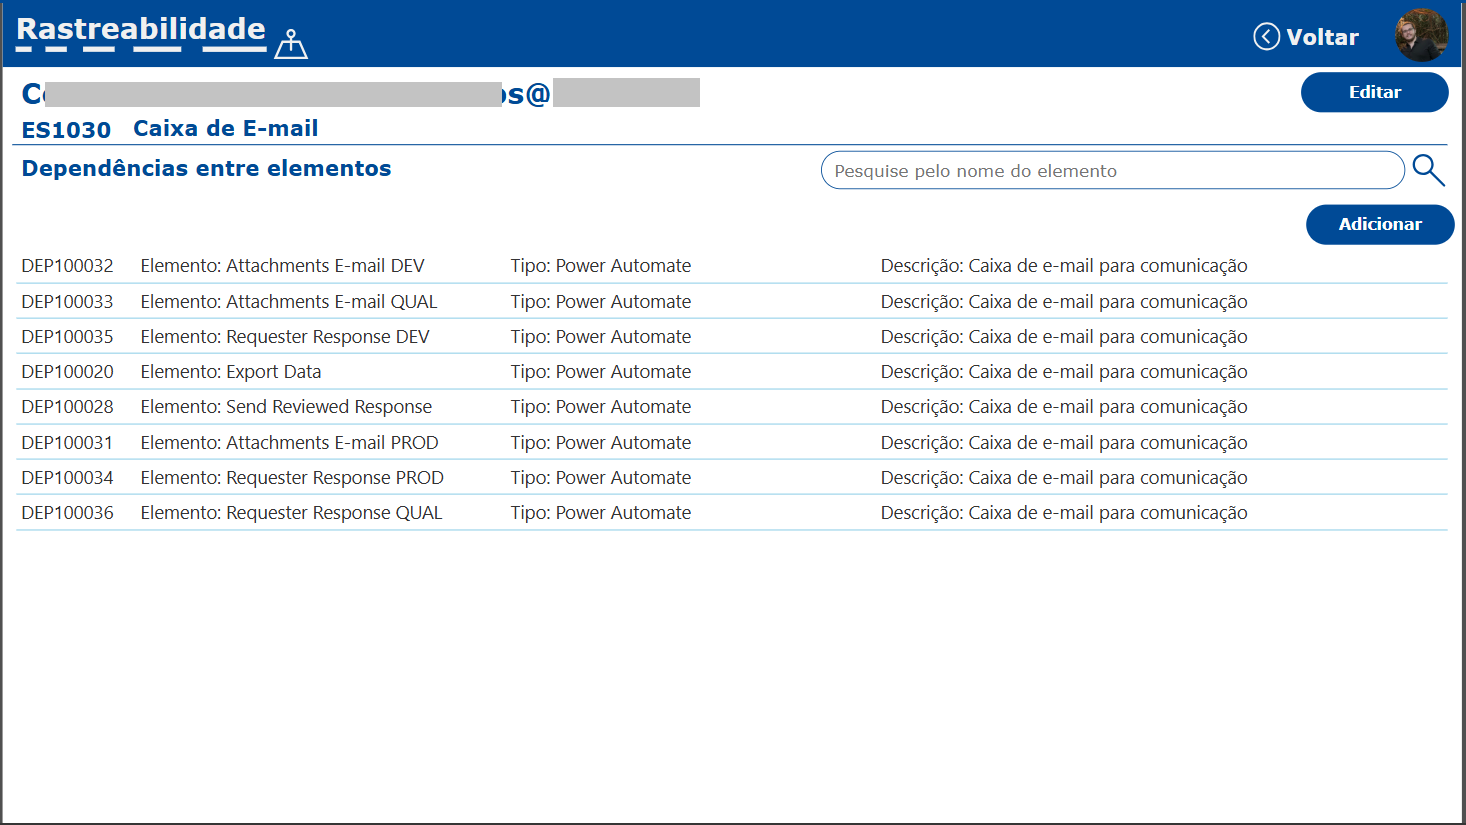
\includegraphics[width=1\textwidth]{./figuras/caixadeEmail.png}
		\caption{Dependências relacionadas ao Cenário 2}
		\label{fig:resultados:caixadeEmail}
	\end{figure}

	\begin{figure}[!h]
		\centering
		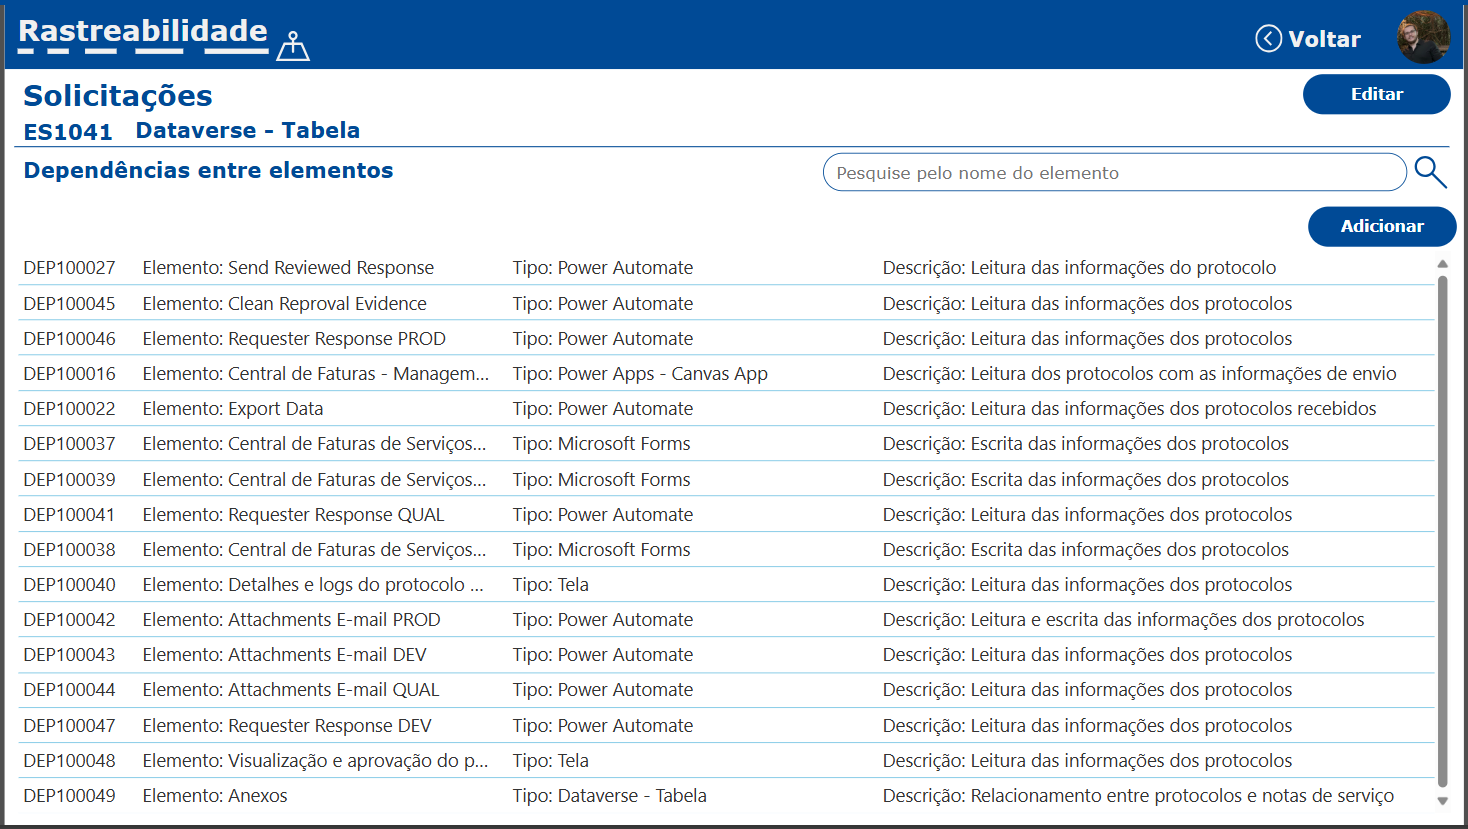
\includegraphics[width=1\textwidth]{./figuras/solicitacoesTabela.png}
		\caption{Dependências relacionadas ao Cenário 3}
		\label{fig:resultados:solicitacoesTabela}
	\end{figure}

	Na Tabela \ref{tab:cenarios_desenvolvimento} podem ser vistos os valores atribuídos a cada cenário antes e depois da apresentação do aplicativo.

	\begin{table}[!htb]
		\centering
		\begin{tabular}{c cc cc cc}
			\toprule
			\textbf{Desenvolvedor} & \multicolumn{2}{c}{\textbf{Cenário 1}} & \multicolumn{2}{c}{\textbf{Cenário 2}} & \multicolumn{2}{c}{\textbf{Cenário 3}} \\
			& Antes & Depois & Antes & Depois & Antes & Depois \\
			\midrule
			1 & 5 & 5 & 1 & 2 & 3 & 5 \\
			2 & 8 & 8 & 1 & 3 & 3 & 8 \\
			3 & 5 & 8 & 1 & 1 & 3 & 5 \\
			\midrule
			Média & 6 & 7 & 1 & 2 & 3 & 6 \\
			Desvio Padrão & 1.73 & 1.73 & 0.00 & 1.00 & 0.00 & 1.73 \\
			\bottomrule
		\end{tabular}
		\caption{Comparativo do esforço alocado em três cenários, antes e depois do uso do aplicativo}
		\label{tab:cenarios_desenvolvimento}
	\end{table}

	Apesar de indicado o desvio padrão para as medidas, não se extrai muita informação dessa comparação visto que foram poucas amostragens de esforço e o valor variou pouco,
	caso um grande número de desenvovedores forem envolvidos faria mais sentido essa métrica. No entanto, ao olharmos para a média das avalições, ou mesmo individualmente por
	desenvolvedor, após a apresentação do aplicativo, na reavaliação, os valores sobem em quase todos os casos individuais e em todos os casos de média.

	Isso mostra um aumento na percepção de esforço a ser empenhado quando se tem clareza das dependências envolvidas na ação que se pretende realizar.

	
	\begin{itemize}		
		\item {\color{red} Sumário dos Resultados: Conclua o capítulo com um sumário dos principais resultados.}
	\end{itemize}